\documentclass[10pt,twocolumn,letterpaper]{article}

\usepackage{btas}
\usepackage{times}
\usepackage{epsfig}
\usepackage{graphicx}
\usepackage{amsmath}
\usepackage{amssymb}


\usepackage{gensymb}
\usepackage{url}
\usepackage{subcaption}
\usepackage{hhline}

\usepackage[breaklinks=true,bookmarks=false]{hyperref}

% Include other packages here, before hyperref.

% If you comment hyperref and then uncomment it, you should delete
% egpaper.aux before re-running latex.  (Or just hit 'q' on the first latex
% run, let it finish, and you should be clear).
%\usepackage[pagebackref=true,breaklinks=true,letterpaper=true,colorlinks,bookmarks=false]{hyperref}

%\btasfinalcopy % *** Uncomment this line for the final submission

\def\btasPaperID{****} % *** Enter the IJCB Paper ID here
\def\httilde{\mbox{\tt\raisebox{-.5ex}{\symbol{126}}}}

% Pages are numbered in submission mode, and unnumbered in camera-ready
\ifbtasfinal\pagestyle{empty}\fi
\begin{document}

%%%%%%%%% TITLE
\title{Deep Convolutional neural network for Fingerprint Pattern Classification}

\author{First Author\\
Institution1\\
Institution1 address\\
{\tt\small firstauthor@i1.org}
% For a paper whose authors are all at the same institution,
% omit the following lines up until the closing ``}''.
% Additional authors and addresses can be added with ``\and'',
% just like the second author.
% To save space, use either the email address or home page, not both
\and
Second Author\\
Institution2\\
First line of institution2 address\\
{\tt\small secondauthor@i2.org}
}

\maketitle
\thispagestyle{empty}

%%%%%%%%% ABSTRACT
\begin{abstract}
   Fingerprints are broadly categorized into five pattern class types.
   Fingerprint pattern classification is useful for quick exclusions and 
   therefore reducing the search space by allowing for search and 
   comparison only within same pattern class type.
   Fingerprint pattern classification can be done by visual examination of
   shape and characteristics of regions of a fingerprint; or using classification 
   algorithms such as neural networks or K-nearest neighbors that are trained 
   to recognize some specified patterns.  To our knowledge, all of the current 
   fingerprint pattern classification algorithms require some processing of 
   fingerprint images to extract features, for example, estimate orientation flow 
   and detect singularities.   In this paper, we present deep learning approach 
   for automated fingerprint pattern type classification without explicit characterization  
   of fingerprint or any feature extraction. 
   This method uses deep convolutional neural network as feature extractor and 
   a Support Vector Machine as classifier.  Our results show that the proposed 
   approach outperforms the state-of-the-art approaches, achieving $98.61\%$ accuracy 
   on NIST SD14 and $100\%$ accuracy on NIST SD4.
\end{abstract}

%-------------------------------------------------------------------------
\section{Introduction}
%!TEX root = main.tex


Fingerprints are ridge and valley patterns presented on the surface of human fingertips.
%
Fingerprints are used to recognize humans for applications such as verifying an identity claim (\textit{i.e.}, one-to-one search to  unlock a smartphone, for example), or identification (\textit{i.e.}, one-to-many search to find a suspect of a crime, for instance).
%
Typically, to query a fingerprint, the system needs to search and compare the query print with the fingerprints stored in a reference (or enrolled) database.  The size of a reference database can be from thousands to hundreds of millions subjects, depending on the application. For example, the Aaddhar project in India has enrolled 111,98,29,743 persons as of February 18, 2017 \cite{aaddhaar}.  
%
As the size of the database grows, the number of comparisons to be made for identification purposes grow, so does the computation time.
%
To mitigate this problem, most fingerprint recognition algorithms first classify a fingerprint into a basic pattern type and then perform fingerprint matching within fingerprints of that type.
%
The major five fingerprint pattern types used today are an extension of the three pattern types (whorl, loop, and Arch) introduced by Henry Faulds (Henry classification system \cite{henry1905classification}) and Sir Francis Galton \cite{galton1892} in late 19th century. These five pattern types are: arch, left Loop, right Loop, tented arch and whorl, see Fig.\ref{fig.fingerprint_classes}.  
%
Because arch and tented arch only accounts for a small portion (around 6\%) in human, some automatic fingerprint identification systems combine these two classes into one class. 

As mentioned above, to manage the computation load, large scale fingerprint identification algorithms employ multi-stage matching whose first step is often filtering based on fingerprint pattern type. As such the accuracy of the fingerprint classification algorithm largely influences the identification accuracy. An error in finger pattern classification will propagate throughout the system, and ultimately result in an recognition error. In this project (paper) we propose an automated fingerprint pattern classification that is not based on feature extraction.

\begin{figure}[!ht]
	\begin{center}
		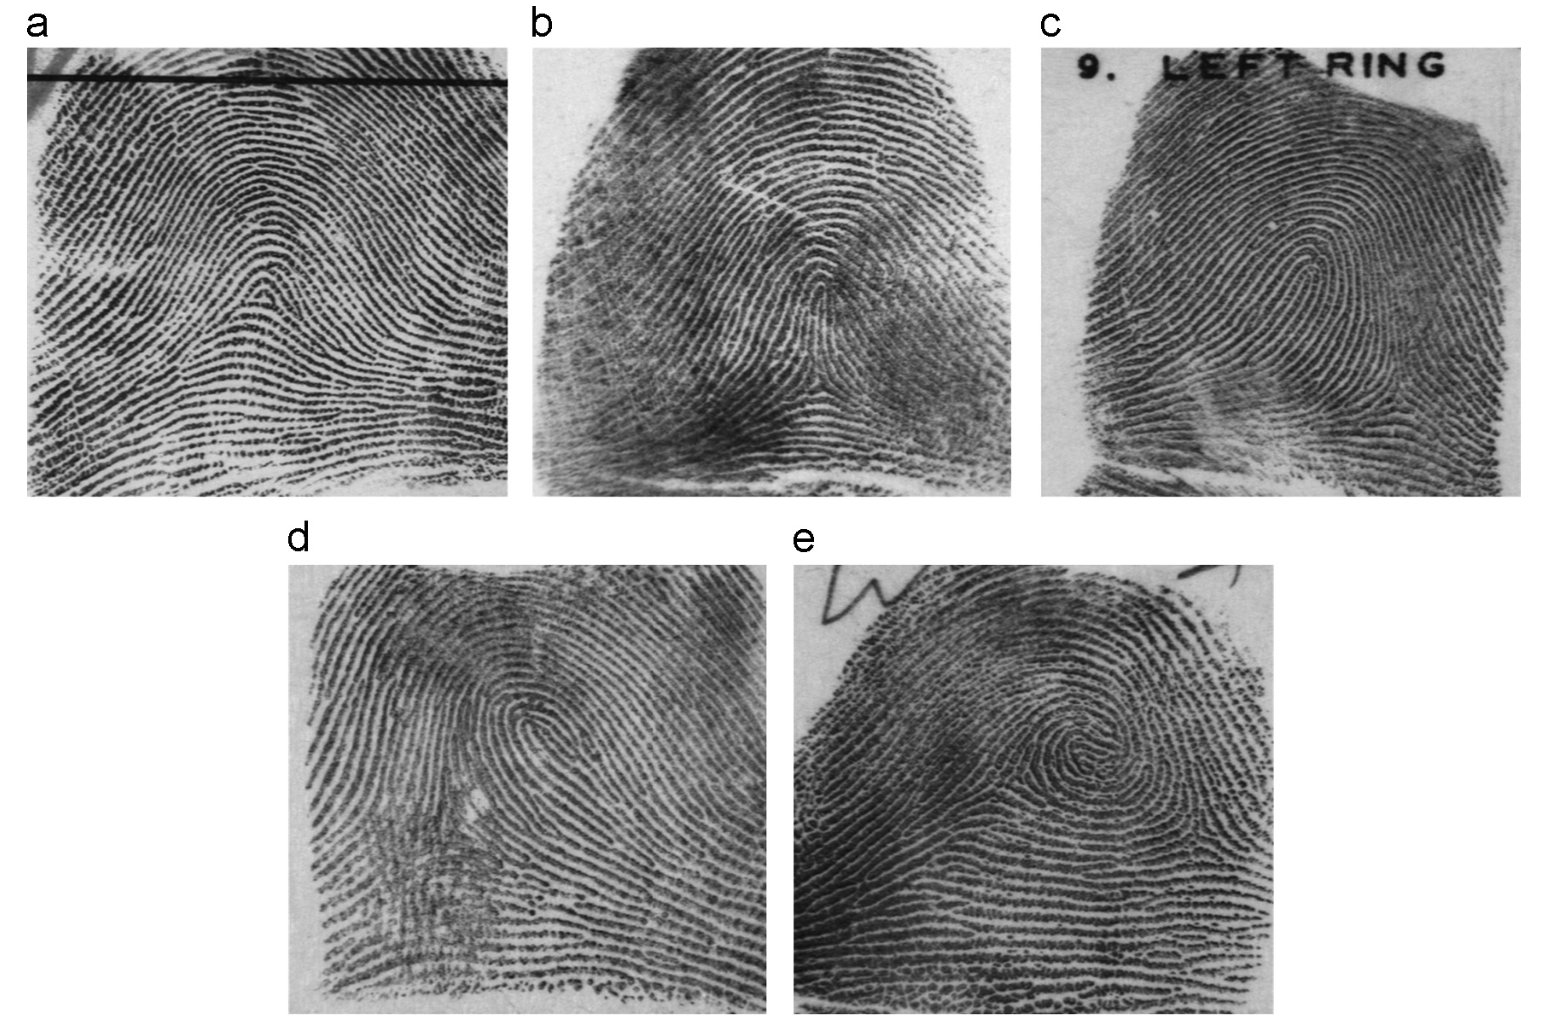
\includegraphics[width=8cm]{fig/Fingerprint_classes.png}
	\end{center}
	\caption{Examples of fingerprint classes\cite{cao2013fingerprint}: (a) Arch (b) Tented Arch (c) Left Loop (d) Right Loop  (e) Whorl.Note  that tented and tented arch are similar.} 
	\label{fig.fingerprint_classes}
\end{figure}



%-----------------------
%\section{Related Work}
%%!TEX root = main.tex

The milestone of the deep reinforcement learning is deep Q-learning(DQN)\cite{mnih2013playing}, a variant of Q-learning, proposed by DeepMind. It is the first deep learning model trying to learn control policies with reinforcement learning. In 2015, DeepMind presented an improved version of DQN\cite{mnih2015human}. Their work outperformed previous algorithms and achieved a capability comparable to that of professional human-being.
%

While DQN performs well in fully-observable environments, it achieves poor result in partially observable environments. To address this problem, Hausknecht and Stone \textit{et al.}~\cite{hausknecht2015deep} introduced the Deep Recurrent Q-Networks(DRQN). The idea is to build a recurrent neural network such as LSTM on top of the DQN model.
%

One drawback of DQN is that it needs to aggregate over time to overcome data non-stationarity. To reduce the overhead caused by experience replay, DeepMind \cite{mnih2016asynchronous} proposed a another paradigm for deep reinforcement learning: multiple agents are running in parallel asynchronously on multiple instances of the environment. Using the paradigm makes Q-learning both efficient and compatible with deep neural network at the same time. They named their best method \textit{asynchronous advantage actor-critic} (A3C). Experiments showed that A3C not only achieved better result but also required less computational cost.
%

%% Alpha go 
 More recently, AlphaGo\cite{brockman2016openai}, which is also developed by DeepMind, defeated Lee Sedol and became the first 'Artificial Intelligence' who beated 9-dan professional human Go player. Behind the AlphaGo is deep neutral network integrated with reinforcement learning improving the play strategy.


%% RDQN 
 RDQN sometimes learn unrealistically high action values because it includes a maximization step over estimated action values, which tends to
 prefer overestimated to underestimated values. This has been demonstrated in some games in the Atari 2600 domain. The idea of double Q-learning algorithm \cite{van2015deep} not only yields more accurate value estimates, but leads to much higher scores on several games. This demonstrates that the overestimations of DQN indeed lead to poorer policies and that it is beneficial to reduce them.


% liyang
% Other application of reinforcement Learning in designing game includes linear evaluation function-based learning of local shape in the game of Go \cite{silver2007reinforcement} and learning control policies for text-based games \cite{narasimhan2015language}

\section{Previous work}
\label{sec_motivtn}

The challenge of classifying fingerprint includes: 
%
1) quality of fingerprints, particularly poor quality; 
%
2) small inter-class dissimilarity and small intra-class similarity; for example, tented arch and loop may look similar; 
%
3) ambiguities in some labels (pattern class; some fingerprints can be classified into multiple classes, or different classes by different fingerprint experts.

Previous work mostly consists of singularity points (core and delta) detection or extracting features such as ridge and orientation flow, or using human markups (or handcrafted features) as the basis for pattern type classification. 
%
Therefore, the accuracy of these methods depends on the goodness (or utility) of the selected features and the precision of the feature extraction portion of the algorithms. Both are sensitive to the noise and the variations of the gray-scale level of the input image.  
%
Using handcrafted features can improve performance.  However, in addition to being burdensome and time consuming, accuracy of handcrafted features cannot be guaranteed due to the existence of noise and poor image quality. 
%
Moreover, their repeatability and reproducibility cannot be guaranteed either, due to inter- and intra-examiners variations \cite{fbiBlackbox}.  
%
Our approach differs from these works in the sense that we aim to use raw images instead of features as input. Convolutional neural network (CNN) has the capability of learning features and it can be directly applied on raw images. CNN also exhibits powerful classification capability in many areas\cite{lecun2015deep}\cite{szegedy2016rethinking}.

%
An overview of related work follows. 
%
Karu and Jain \cite{karuJain1996} presented a rule-based classifier based on extracting singular points. 
%
Fitz and Green \cite{FitzGreen1996} used a Hexagonal Fourier Transform to classify fingerprints into whorls, loops and arches. 
%
Jain \textit{et al.} \cite{JainSalil1999} used a bank of Gabor filters to compute a feature vector (FingerCode) and then used a K-nearest neighbor classifier and a set of neural networks to classify a feature vector into one of the five fingerprint pattern classes.
%
Cappelli \textit{et al.} \cite{cappelli1999} partitioned a fingerprint directional image into ``homogeneous'' connected regions according to the fingerprint topology, resulting in a synthetic representation which is then used as a basis for the classification.
%
Bernard \textit{et al.} \cite{Bernard2001} used the Kohonen topologic map for fingerprint pattern classification. 
%
Kai Cao \textit{et al.}\cite{cao2013fingerprint} proposed to extract fingerprint orientation feature and used a hierarchical classifier for classification.
%
Ruxin Wang \textit{et al.} \cite{wang2014fingerprint} also used orientation filed as features. By adopting a stacked autoencoder, they achieved 93.1\% in four-class classification.
%%
 


%-----------------------


%\section{Proposed research}
%%!TEX root = main.tex

In this project, we aim to develop and implement a deep learning algorithm that takes a fingerprint image as an input and classify it into one of the five pattern class types of a) Arch; b) Tented Arch; c) Left Loop; d) Right Loop; or e) Whorl. 

\subsection{Feature Extraction}
%
We will first apply raw fingerprint images to train a CNN for classification. The outputs of some intermediate layer of CNN will be used as features for possibly a support vector machine classifier.

For CNN architecture, we will first use canonical architecture (such as 5 \textit{convolutional} + 3 \textit{fully-connected} in \textit{AlexNet} \cite{krizhevsky2012imagenet}).
%
We will then modify the CNN architecture to improve the performance.
%
\subsection{Classifier}
%
We will consider two classifiers. The first one is the prediction layer of CNN. The values in last layer indicates the predicted probabilities of each class.
%
The second one is support vector machine (SVM) whose input features comprise of the CNN’s middle or last layers.

\subsection{Data Augmentation}

%
To further improve the performance, we will use data augmentation technique to generate more training samples in order to increase the generalization ability of our model. 
%
The augmentation methods include image rotation, resizing and translation.

\subsection{Multi-Task Learning}

Multi-Task Learning (MTL)\cite{caruana1998multitask} aims to improve the performance of multiple classification tasks by learning them jointly.
%
In MTL, some tasks can benefit from auxiliary information which is introduced by other tasks and the performance is improved\cite{zhang2016learning}.
%
In our project, the network is trained to perform both the primary task (fingerprint type classification) and one or more auxiliary tasks. 
%
The classification task is expected to benefit from the auxiliary task by jointly training them together.
%
This process can also be viewed as incorporating human knowledge into to training procedure.

To obtain labels for auxiliary tasks, we will use existing methods. For example, orientation flow estimation in \cite{NFIQ}.

%\label{sec_plan}

%\section{Dataset}
%
In this project, we will use NIST Special Database 4 \cite{nist-db-4} for our experiments. Some samples can be seen in Fig.\ref{fig.fingerprint_classes}.
%
The NIST database of fingerprint images contains 2000 8-bit gray scale fingerprint image pairs, totally 4000 images.
%
Each image is 512-by-512 pixels with 32 rows of white space at the bottom and classified using one of the five following classes: Arch, Left and Right Loops, Tented Arch, Whorl.
%
Each of the five classes has 400 pairs. Each of the fingerprint pairs are two completely different rollings of the same fingerprint.
%\label{sec_dataset}

%-----------------------
\section{Methodology}
\label{sec_method}
%!TEX root = main.tex

Figure\ref{fig.method} illustrates our technical approach.   
%
The top row shows the steps of the training process.  First, training images are preprocessed using data augmentation techniques to increase data diversity. 
The augmented data are fed into deep ConvNet for training. The trained deep ConvNet then serves as a feature extractor for a SVM which uses the deep features from the trained deep ConvNet as input, and is trained to classify the pattern type.
%
During the testing, shown in the bottom row of Figure\ref{fig.method}, testing images are fed into the trained deep ConvNet for deep features extraction. These intermediate deep features are used as input features to the trained SVM. The output of the SVM is our final pattern class prediction.


\begin{figure}[!ht]
	\begin{center}
		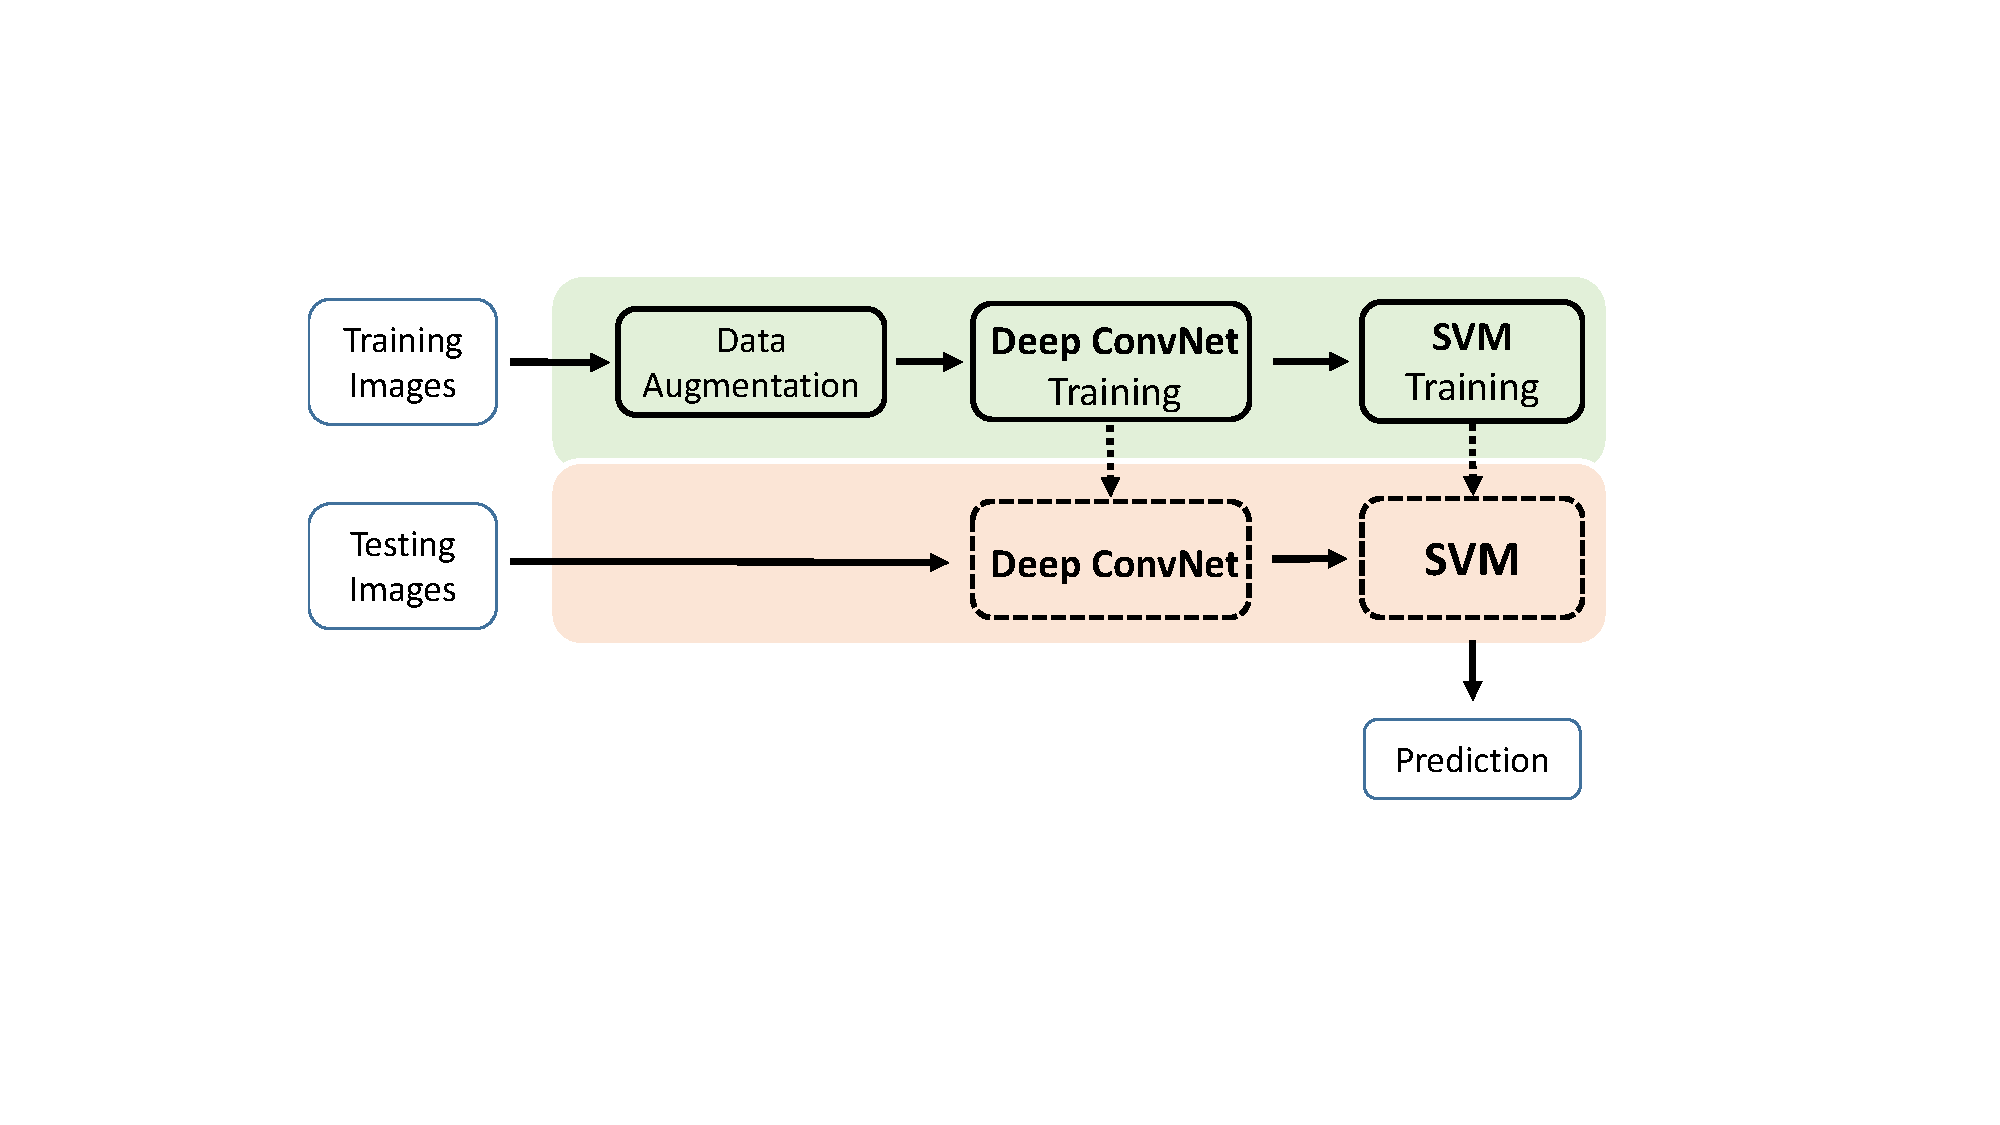
\includegraphics[scale=0.38,clip=true,trim = 50mm 55mm 50mm 50mm]{fig/figs/method_overview.pdf}
	\end{center}
	\caption{Overview of proposed approach.} 
	\label{fig.method}
\end{figure}

%-------------------------
\subsection{Deep ConvNet Architecture}
\label{sec_cnn}
Our proposed network architecture (Figure \ref{fig.cnn_arch})  is based on deep residual network proposed by Kaiming He \textit{et al.}\cite{he2016deep}. Deep residual  network has been proven to outperform other deep plain networks because it addresses the degradation problem by reformulating the layers as learning residual functions instead of learning unreferenced functions. 
%
Table\ref{tab.cnn_params} summarizes the details of our network. The input size of our deep ConvNet is $512\times512$ and the number of channels is $1$.
The first two layers of our network are convolutional layers which has 96 $7\times7$ filters and the stride is 2. The third layer has 64 $7\times7$ filters and the stride is 2. 
%
\textit{conv4}, \textit{conv5}, \textit{conv6} and \textit{conv7} are composed of residual building blocks. Specifically, there is a max pooling layer before  \textit{conv4}. The parameters inside the brackets specify the residual building block size. 
%
The multiplier after bracket specifies the multiplicity of the that block in that layer.  More details and explanations regarding network architecture can be found in \cite{he2016deep}. 
%
The global pooling layer in \textit{conv8} generates $1\times1,2048$ output and the last layer uses 5 $1\times1$ filters to generate the final prediction. 
%
The number of parameters of proposed deep ConvNet is $24.26$ million. 
%
We use Relu\cite{nair2010rectified} as intermediate activation function.
%

The novelty of our network is that we use $512\times512$ as network input size. This preserves the detail of fingerprint information to the extent possible. 
%
However, the larger the size of input images, the larger the computational cost.  We empirically searched for the optimal input image size and we found that the performance drops as the size gets smaller, and it drops significantly for images smaller than $224\times224$ -- as shown in Figure\ref{fig.resize_examples}, down-sampling the images to $224\times224$, results in loss of information content of prints and reduces the clarity of ridge details and deltas and cores. 
%
Therefore we decided against significant down sampling.  
%
We also ruled out cropping or segmenting the fingerprint portion of an image, that is removing background and non-fingerprint portion of images to get smaller images, because of its requiring to employ a segmentation algorithm and reliance on the accuracy of the segmentation algorithm -- recall that one of our objective has been to avoid fingerprint processing and characterization.
%
After careful visual inspection of fingerprint images of different sizes, we decided to use $512\times512$ pixels as input size for the following reasons. 
%
First, sufficient fingerprint detail is preserved at this size. Second, it is a reasonable size for rolled fingerprints. Finally, it is the original image size of one of the datasets we used, which is NIST SD4.
%
To remedy the huge computational cost and high memory usage during the training, we added \textit{conv1} and \textit{conv2} with stride 2 to down-sample the input images. As shown in Table.\ref{tab.cnn_params}, after \textit{conv2}, the feature map size is $128\times128, 96$. So, the spatial size is reduced (from $512 \times 512$ to $128 \times 128$) and spatial information is stored in the increased channels (from $1$ to $96$).

%
\begin{figure}[!ht]
	\begin{center}
		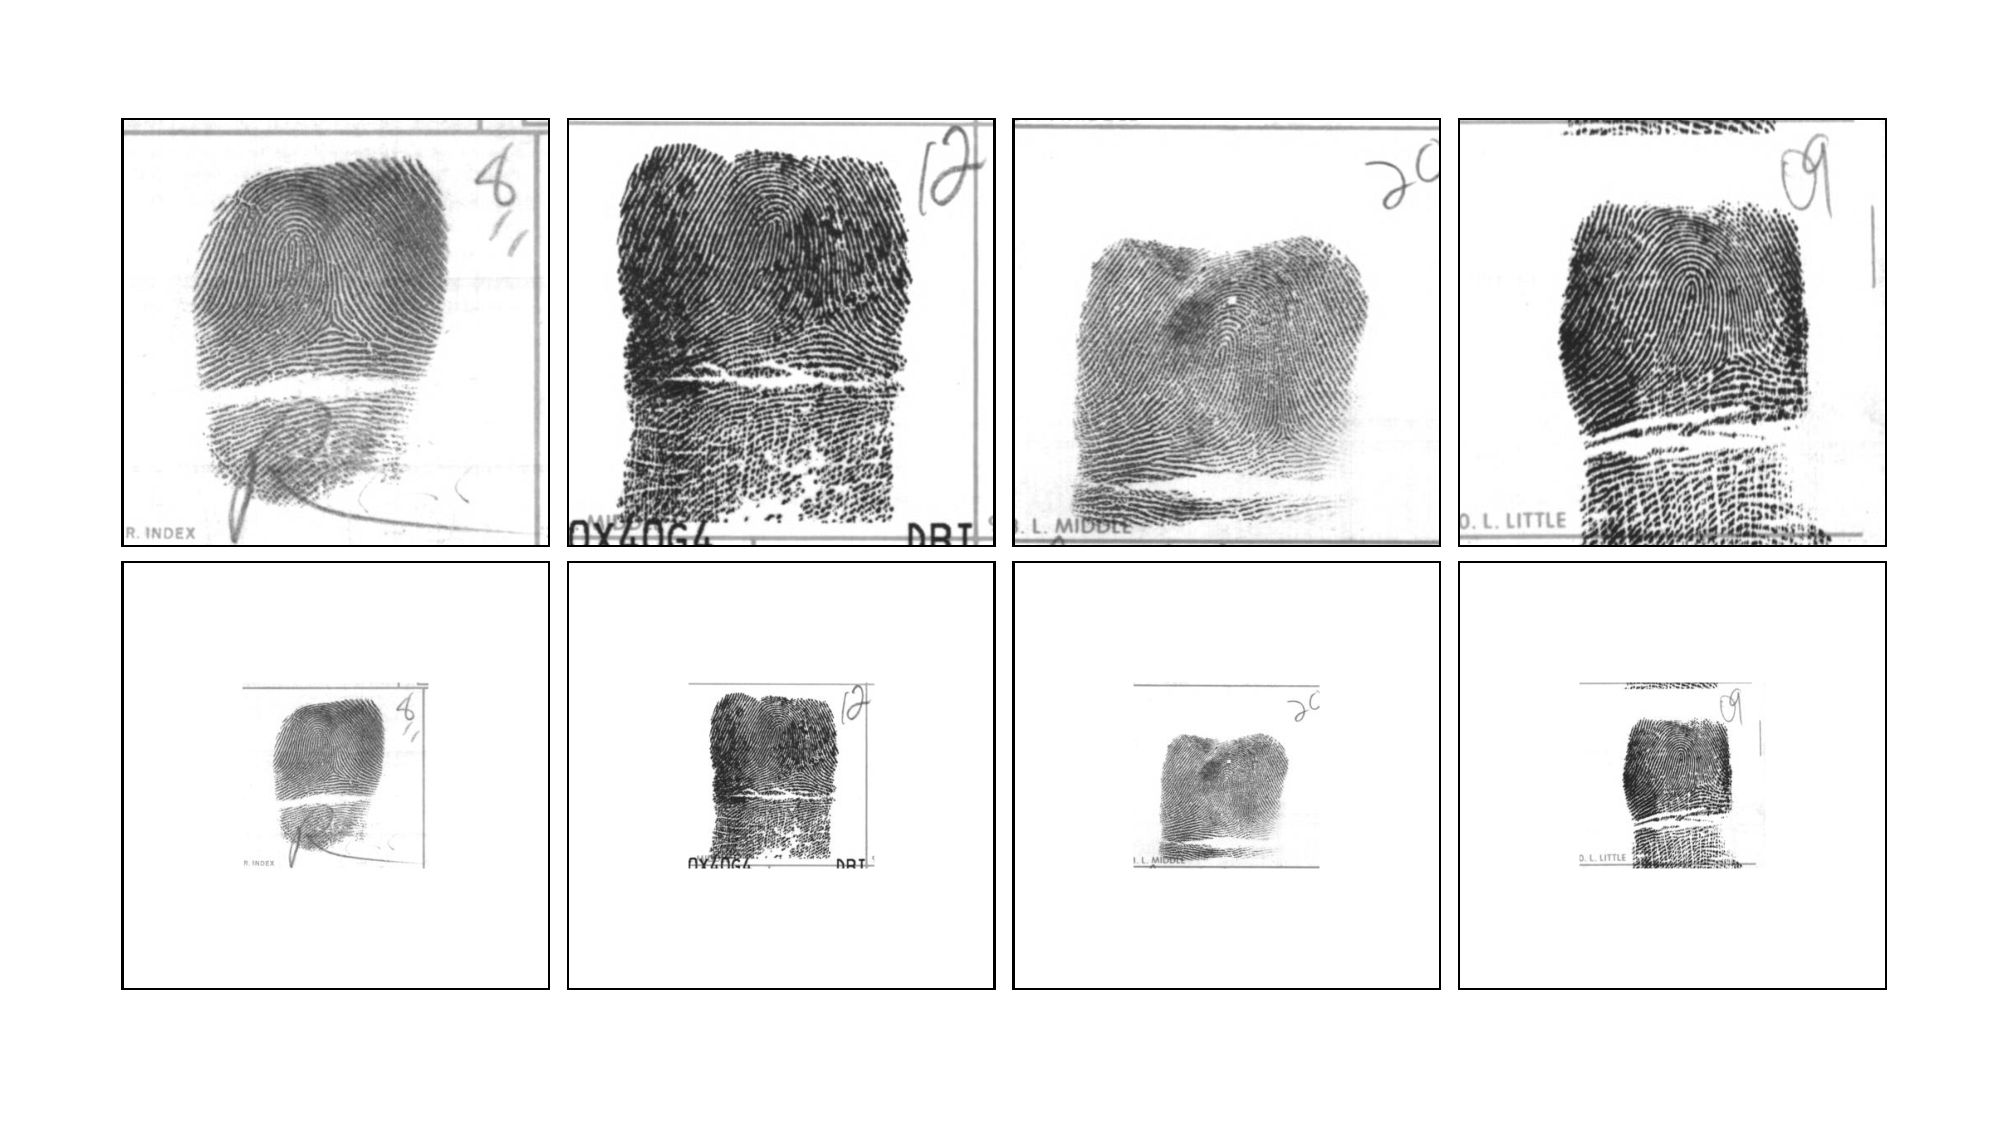
\includegraphics[scale=0.28,clip=true,trim = 20mm 15mm 10mm 10mm]{fig/figs/resize_examples.pdf}
	\end{center}
	\caption{Example images from NIST SD14 with different spatial sizes. The top row images are $512\times512$ and the bottom row are $224\times224$. Ridges of top images are more distinguishable than that of bottom images. } 
	\label{fig.resize_examples}
\end{figure}
%
%
\begin{figure*}[!ht]
	\begin{center}
		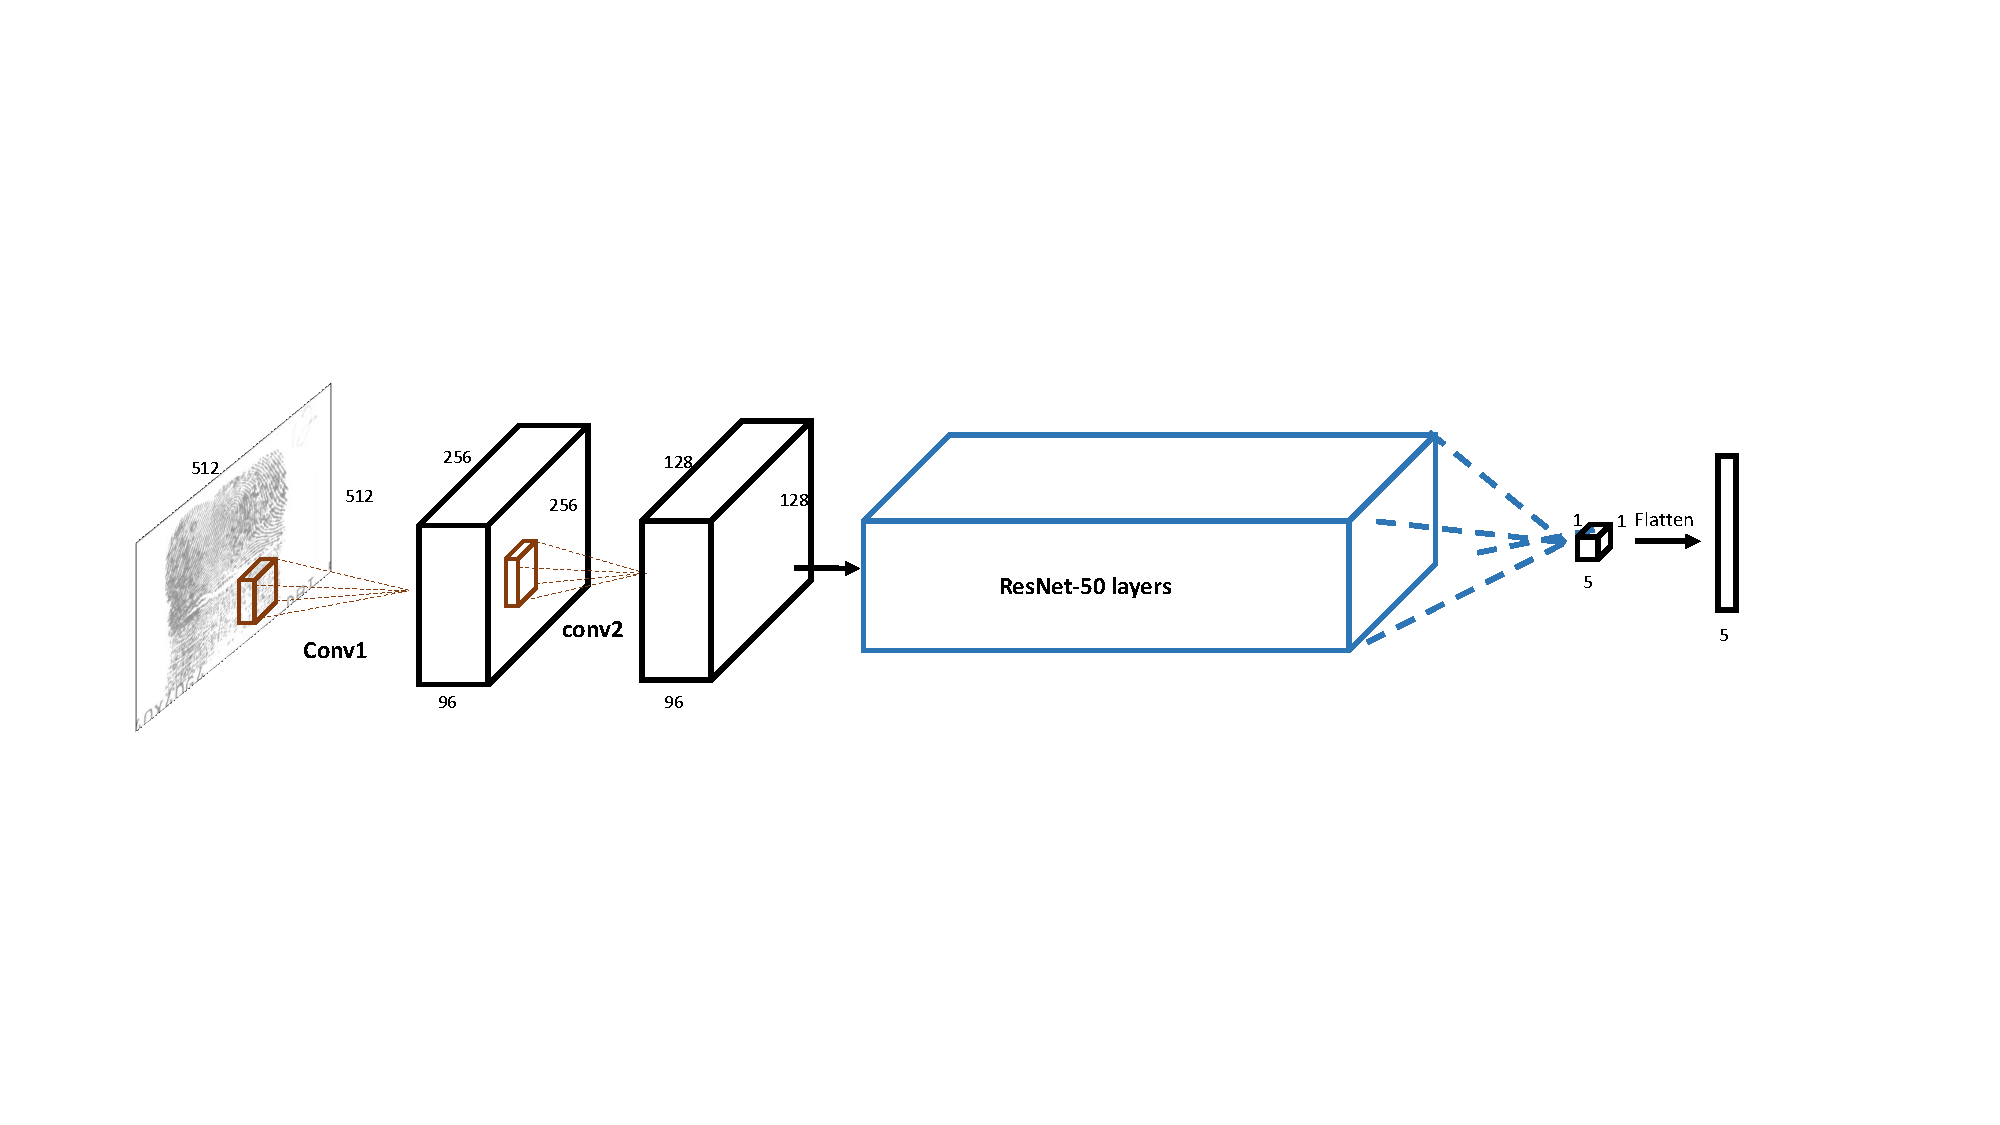
\includegraphics[scale=0.65,clip=true,trim = 20mm 65mm 40mm 65mm]{fig/figs/cnn_arch.pdf}
	\end{center}
	\caption{Architecture of proposed CNN.} 
	\label{fig.cnn_arch}
\end{figure*}


\begin{table}[!ht]
	\centering
	\caption{Detail of proposed deep ConvNet. The format is inspired by \cite{he2016deep}}
	\label{tab.cnn_params}
	\begin{tabular}{l}
		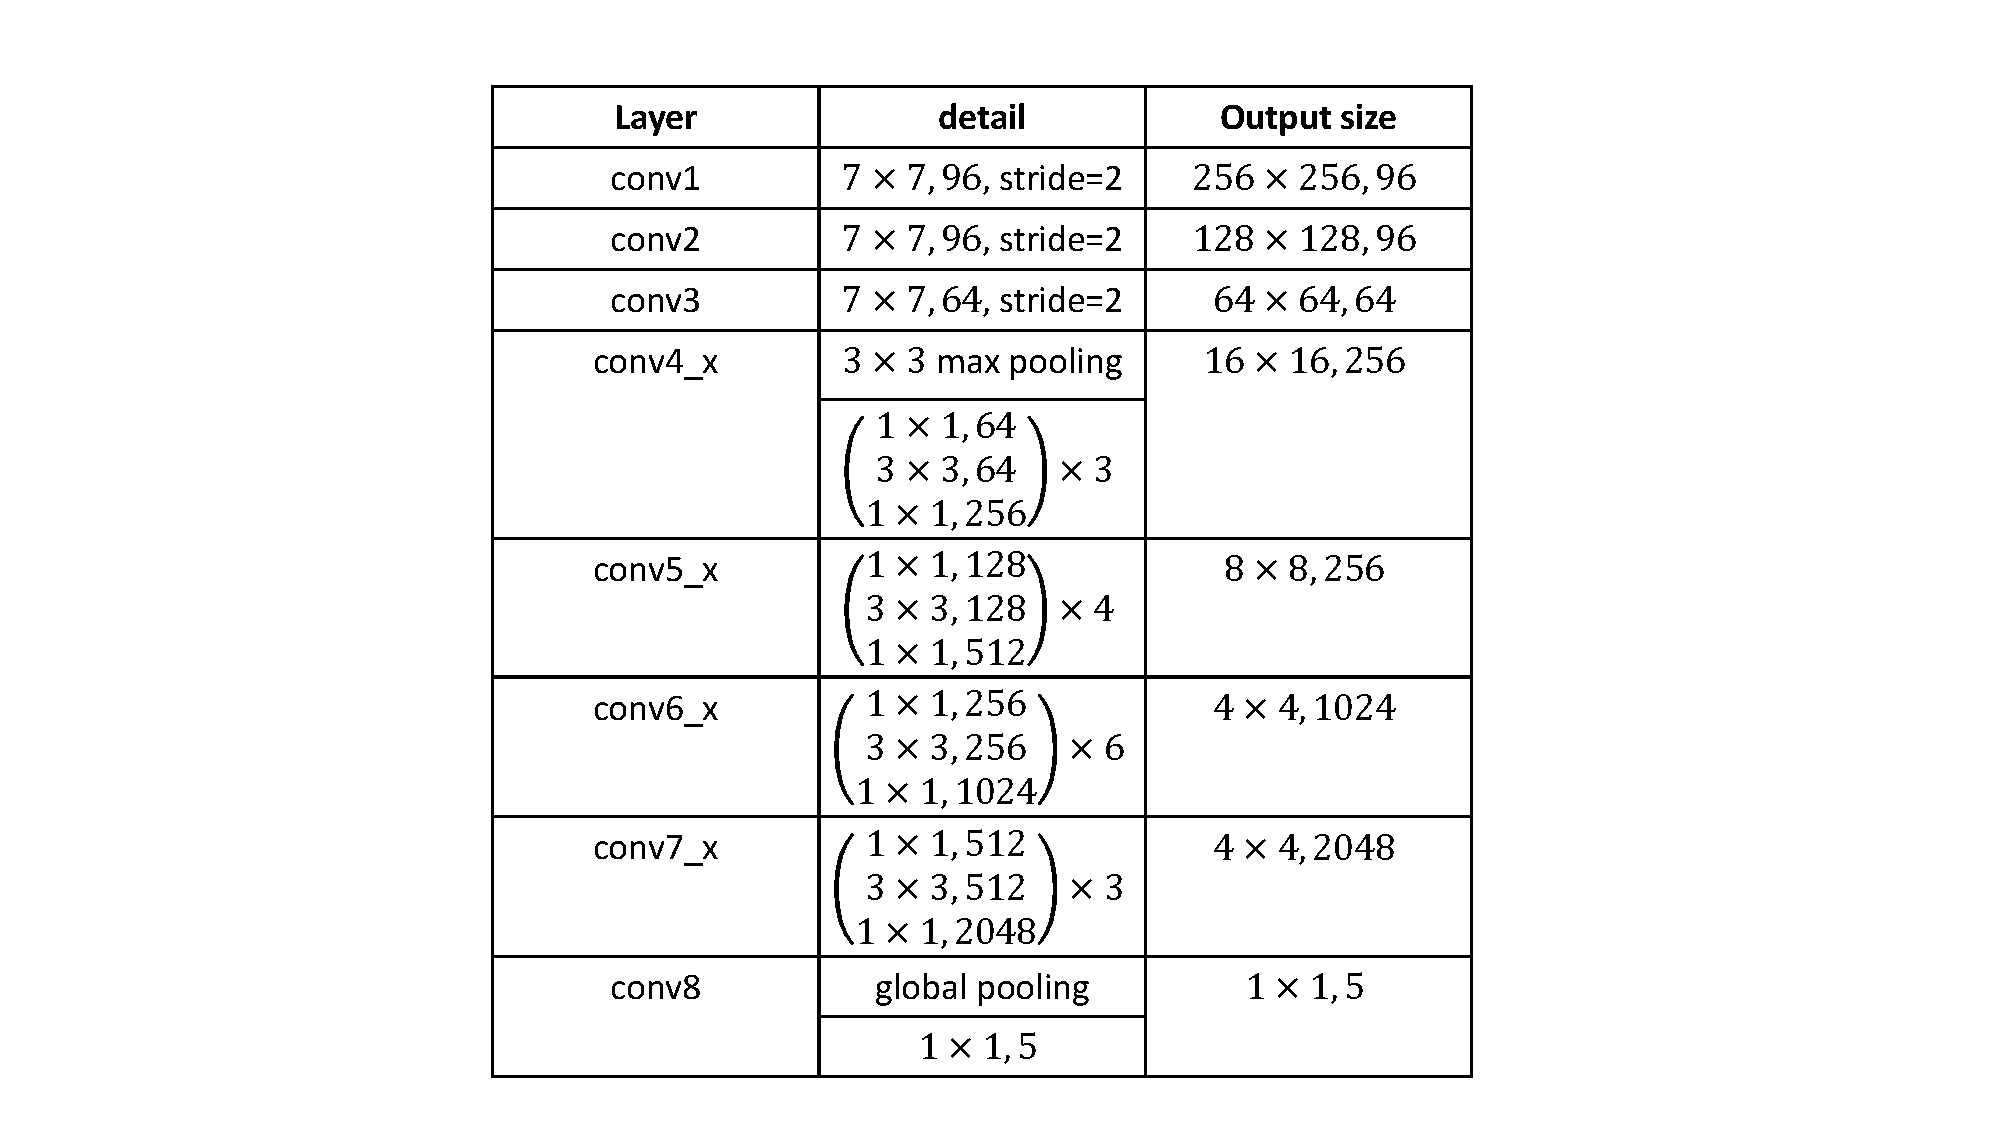
\includegraphics[scale=0.45,clip=true,trim = 78mm 5mm 70mm 5mm]{fig/figs/cnn_table.pdf}
	\end{tabular}
\end{table}

%-------------------------
\subsection{Data Augmentation}
\label{sec-dataAug}
Fingerprint images exhibit a wide range of location, rotation, brightness and contrast. To enhance the generalization ability of our ConvNet, we adopt data augmentation techniques to increase the data diversity.
	
To augment training dataset, we applied below augmentation techniques:

\begin{enumerate}

	\item Random Cropping. The input images are first resized to $532 \times 532$. We randomly cropped a $512\times512$ region from the resized images.
	\item Random Rotation. We randomly rotate the input images by $\omega$ degrees where $\omega \sim uniform (-30\degree, 30\degree)$.
	\item Random Brightness.  Random brightness change is performed on the input images. The gray scale of the input images $I$ are change to $I + \delta$ where $\delta$ is  sampled from $uniform (-50, 50)$.
	\item Random Contrast. We randomly change the contrast of images. The contrast factor is sampled from $uniform (0.4, 1.6)$.

\end{enumerate}

%-------------------------
\subsection{SVM}
\label{sec_svm}
We examined two scenarios: the deep ConvNet is trained for feature extraction and classification and another scenario where the deep ConvNet only serves as a feature extractor and a non-linear SVM is trained as classifier. For the latter case, the kernel is radial basis function(RBF). The gamma of RBF kernel  is set to be $\frac{1}{n}$ where $n$ is the feature dimensionality. The penalty for error term $C$ is set to be $1.0$. 
%
We use the output of  conv7\_x as features. Therefore, each sample is represented by a feature vector $x \in \mathbb{R}^d$ where $d=4*4*2048=32768$. The output of SVM is the predicted label $\hat{y} $ indicating one of the fingerprint pattern class types.
%









%-----------------------
\section{Experiments}
\label{sec_exp}
%!TEX root = main.tex

\subsection{Dataset}

In this project, we  use NIST Special Database 4 \cite{nist-db-4} and NIST Special Database 14 \cite{nist-db-14} for our experiments. 
%
The NIST SD4 contains $2000$ 8-bit gray scale fingerprint image pairs, totally 4000 images.
%
The size of each image is $512\times512$ and each image is classified using one of the five following classes: Arch, Left and Right Loops, Tented Arch, Whorl.
%
Each of the five classes has 400 pairs(800 images). Each of the fingerprint pairs are two completely different rollings of the same fingerprint.

%
The NIST SD14 contains $27000$ 8-bit gray scale fingerprint image pairs. There are 2700 subjects in this dataset and each subject has 10 fingerprint samples pairs. The size of each image is  $768\times832$. To fit in our network, we centrally crop $768\times768$ from the samples and resize them into $512\times512$. 
%
The distribution of fingerprint classes is as shown in Table.\ref{tab.sd14_dist}. We can see that unlike NIST SD4, Arch and Tented Arch samples are only a small portion of the NIST SD14.


\begin{table}[!ht]
	\centering
	\caption{Class Distribution of NIST SD14.}
\label{tab.sd14_dist}
	\begin{tabular}{|c|c|c|c|c|}
		\hline
		\textbf{Arch} & \textbf{Left Loop} & \textbf{Right Loop} & \textbf{\begin{tabular}[c]{@{}c@{}}Tented \\ Arch\end{tabular}} & \textbf{Whorl} \\ \hline
		3.6\% & 31.9\% & 30.5\% & 3.2\% & 30.8\% \\ \hline
	\end{tabular}
\end{table}

\subsection{Experimental Setup}
We use a i7-5930K desktop with 32GB memory and a Nvidia GTX TITAN X GPU for experiments.
%
Typically, we use Tensorflow 1.0.1 as the deep learning library and Adaptive Moment Estimation(Adam\cite{kingma2014adam}) as the optimization algorithm. The learning rate is 0.0001. We also use $\ell_2$ regularization with 0.0001 weight decay rate. The batch size is 32. 
%
We evaluate our approach on NIST SD4 and NIST SD14 respectively. Each experiment is trained for $20k$ steps.


%
For NIST SD14 experiments, we use the samples of $80\%$ subjects for training, totally 2160 subjects with $43200$ images. Among these $432000$ images, $36$ of them have labels that do not belong to the 5 classes. These $36$ images are discarded. 
The remained data of $20\%$ subjects are used for testing, totally $10800$ images. $9$ of these images are discarded due to the same reason above.
%

For NIST SD4 experiments,  we adopt two evaluation protocols. 
%
The first protocol is cross-sample for fair comparison with other works, where we use all the first samples in each fingerprint pair as training set and all the second samples as testing set.
%
The second protocol is cross-finger, where we use 50\% fingers for training and 50\% for testing to ensure the same finger does not existing in training and testing set at the same time. To improve the performance for NIST SD4, We use NIST SD14 data to pre-train the model.
 

In addition to 5-class fingerprint classification, we also evaluate our SVM performance on 4-class fingerprint classification because 4 class classification are also used in other studies. 
%
To achieve 4-class classification, we merge Tented Arch class into Arch class when training SVM.

\begin{figure*}[!ht]
	\begin{subfigure}[b]{0.25\textwidth}
		\centering
		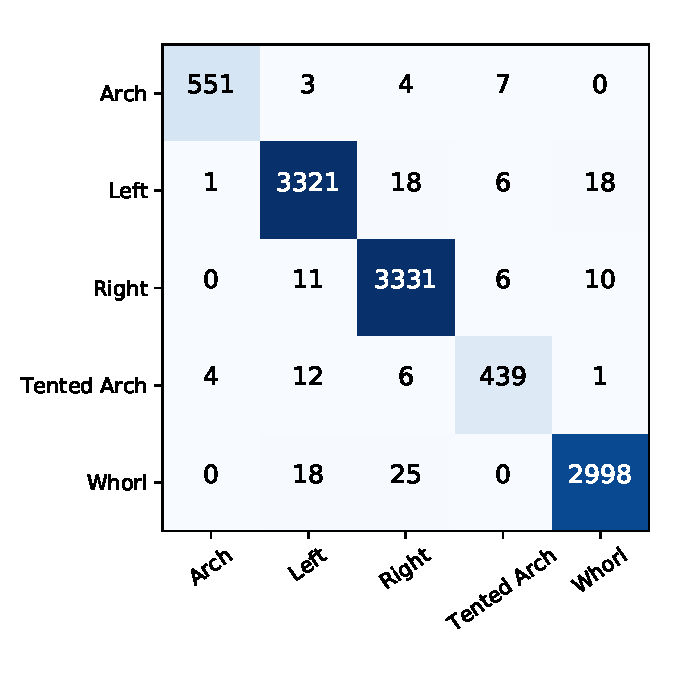
\includegraphics[width=\linewidth]{fig/figs/confusion_matrix_svm_sd14.pdf}
		\caption{SVM for NIST SD14 }
		\label{fig.cnf_matrix_5class.svm_sd14}
	\end{subfigure}%
	\begin{subfigure}[b]{0.25\textwidth}
		\centering
		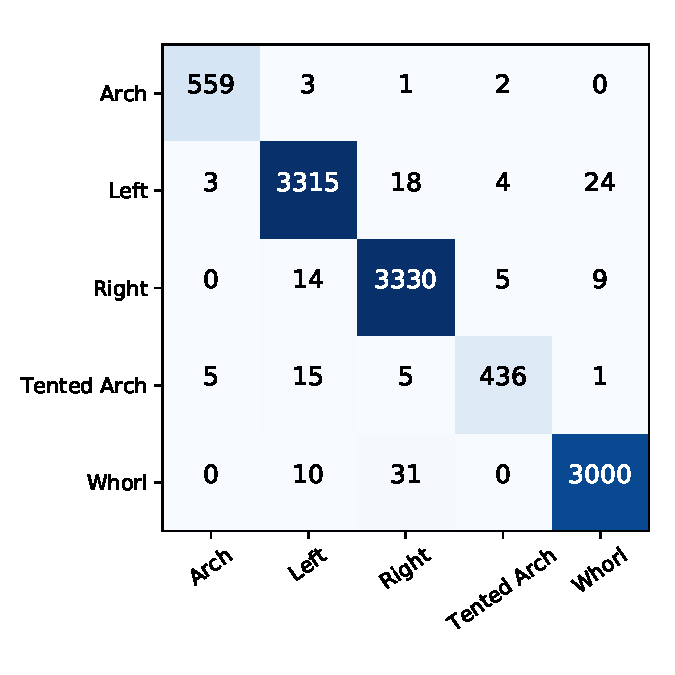
\includegraphics[width=\linewidth]{fig/figs/confusion_matrix_net_sd14.pdf}
		\caption{ConvNet for NIST SD14 }
		\label{fig.cnf_matrix_5class.net_sd14}
	\end{subfigure}%
	\begin{subfigure}[b]{0.25\textwidth}
		\centering
		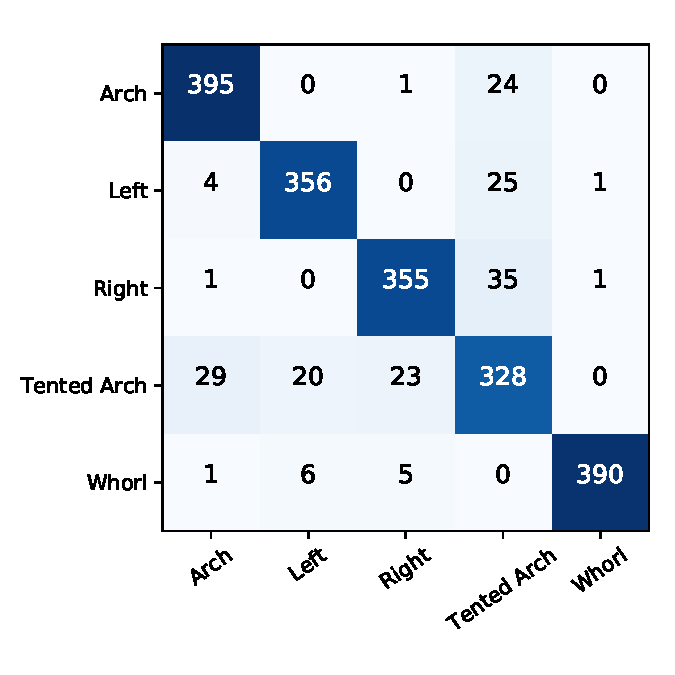
\includegraphics[width=\linewidth]{fig/figs/confusion_matrix_svm_sd4_cross_subject.pdf}
		\caption{SVM for NIST SD4 }
		\label{fig.cnf_matrix_5class.svm_sd4}
	\end{subfigure}%
	\begin{subfigure}[b]{0.25\textwidth}
		\centering
		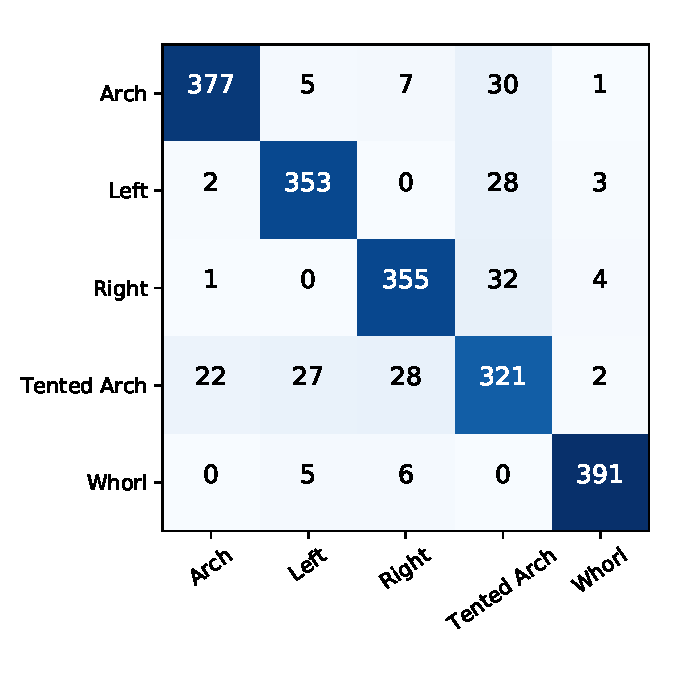
\includegraphics[width=\linewidth]{fig/figs/confusion_matrix_net_sd4_cross_subject.pdf}
		\caption{ConvNet for NIST SD4 }
		\label{fig.cnf_matrix_5class.net_sd4}
	\end{subfigure}
	\caption{Confusion Matrices for 5-class classification}\label{fig.cnf_matrix_5class}
\end{figure*}

\begin{figure}[!ht]
	\begin{subfigure}[b]{0.25\textwidth}
		\centering
		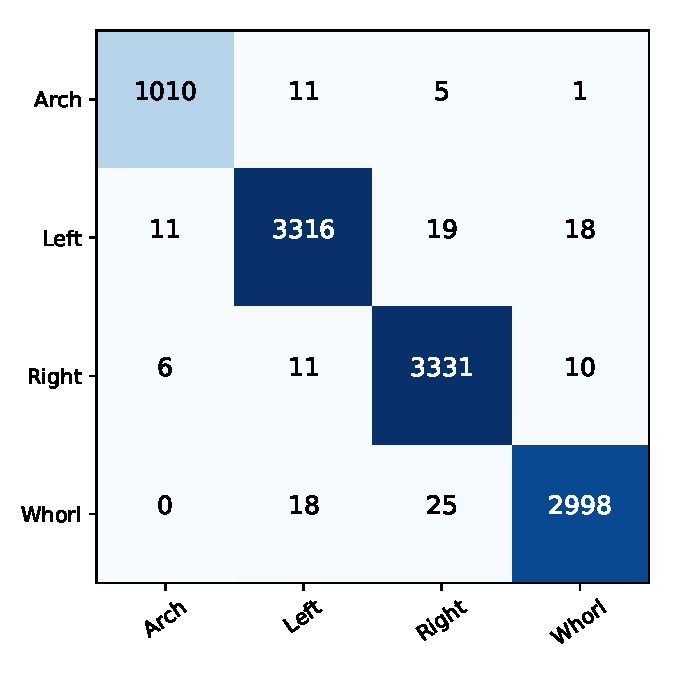
\includegraphics[width=\linewidth]{fig/figs/confusion_matrix_svm_sd14_4class.pdf}
		\caption{SVM for NIST SD14 }
		\label{fig.cnf_matrix_4class.svm_sd14}
	\end{subfigure}%
	\begin{subfigure}[b]{0.25\textwidth}
		\centering
		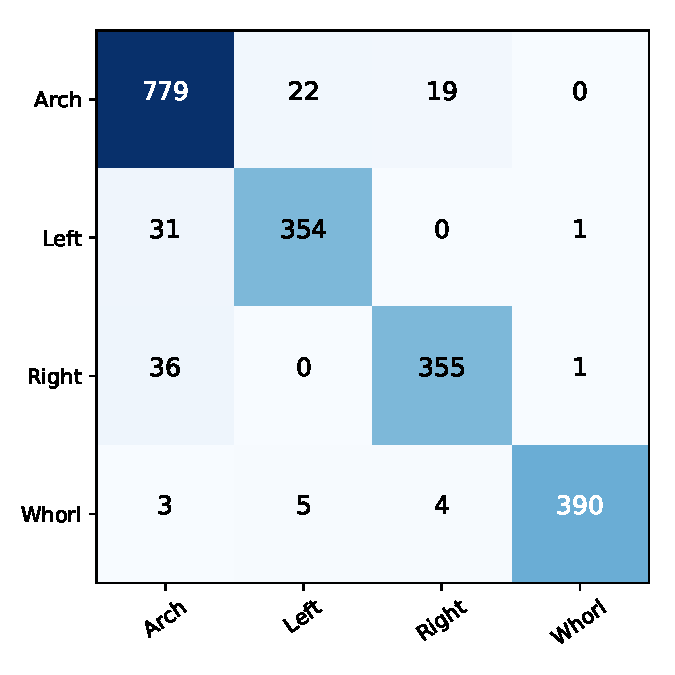
\includegraphics[width=\linewidth]{fig/figs/confusion_matrix_svm_sd4_4class_cross_subject.pdf}
		\caption{SVM for NIST SD4}
		\label{fig.cnf_matrix_4class.svm_sd4}
	\end{subfigure}%

	\caption{Confusion Matrices for 4-class classification}\label{fig.cnf_matrix_4class}
\end{figure}

\subsection{NIST SD14 result}
The result for NIST SD14 is shown in Table\ref{tab.SD14_result}.
%
In addition to report SVM performance, we also report the performance when ConvNet is used as classifier. 
%
As we can see, both ConvNet and SVM achieve the same accuracy ($0.9861$) for 5-class classification. 
%
However, ConvNet performs slightly better in terms of average precision, recall rate and F1 score.
%
For 4-class classification, the 4-class SVM achieves $0.9875$ accuracy.

For 5-class classification, the confusion matrix is shown in Figure.\ref{fig.cnf_matrix_5class.svm_sd14} and Figure.\ref{fig.cnf_matrix_5class.net_sd14}.
For 4-class classification, the confusion matrix is shown in Figure.\ref{fig.cnf_matrix_4class.svm_sd14}. 
%
As we can see, the number of Arch and Tented Arch samples are relatively small compared to other classes.
%
However, our proposed approach can still achieve high accuracy despite the unbalanced distribution of fingerprint types.
%
Though computation based on Figure.\ref{fig.cnf_matrix_5class.svm_sd14}, we can see that Tented Arch achieves the lowest precision (0.959) and recall rate(0.950) due to lack of training samples and label ambiguity. 
%
Based on Figure.\ref{fig.cnf_matrix_4class.svm_sd14}, both the precision and recall rate of Arch increases to $0.98$, indicating many mis-classified samples can be eliminated by combing Arch and Tented-Arch classes.


\begin{table}[!ht]
	
	\centering
	\caption{ Experiment results for NIST SD14. In column 4, 5 and 6, we also report the average precision, recall and F1 score for all predicted classes. }
	\label{tab.SD14_result}
	\scalebox{0.87}{
	\begin{tabular}{|c|c|c|c|c|c|}
		\hline
		\textbf{method} & \textbf{\begin{tabular}[c]{@{}c@{}}\# of \\ classes\end{tabular}} & \textbf{accuracy} & \textbf{\begin{tabular}[c]{@{}c@{}}average \\ precision\end{tabular}} & \textbf{\begin{tabular}[c]{@{}c@{}}average\\  recall\end{tabular}} & \textbf{\begin{tabular}[c]{@{}c@{}}average \\ F1 score\end{tabular}} \\ \hline
		ConvNet & 5 & 0.9861 & 0.9843 & 0.9793 & 0.9817 \\ \hline
		SVM & 5 & 0.9861 & 0.9822 & 0.9781 & 0.9801 \\ \hline
		SVM & 4 & 0.9875 & 0.9869 & 0.9867 & 0.9868 \\ \hline
	\end{tabular}
}
\end{table}

\subsection{NIST SD4 Result}

The result for NIST SD4 is shown in Table\ref{tab.SD4_result}.
%
We have three observations from Table\ref{tab.SD4_result}.
%
First, in both protocol, our proposed SVM performs better than ConvNet not only in accuracy but also in average precision, recall rate and F1 score. 
%
In cross-sample protocol, the accuracy of 5-class SVM is $0.9275$, which is $0.006$ higher than 5-class ConvNet. In cross-finger protocol, the accuracy of 5-class SVM is $0.912$, $0.014$ higher than 5-class ConvNet.
%
Second, there is a performance drop in cross-finger compared to cross-sample. For 5-class ConvNet, the accuracy drops $0.023$. For 5-class SVM, the accuracy drops $0.015$. For 4-class SVM, the accuracy drops $0.011$. 
%
SVM suffers the smaller performance drop than ConvNet if cross-finger protocol is used.
%
The performance drop is small, indicating the generalization ability of our proposed method.
%
Third, the accuracy is improved if Tented Arch and Arch are combined into one-class. The accuracy of 4-class SVM is $0.022$ higher than 5-class SVM in cross-sample and $0.027$ higher in cross-finger. This indicates many mis-classified samples can be eliminated by combing Arch and Tented-Arch classes, as in NIST SD 14.

For 5-class classification using cross-finger protocol, the confusion matrices are shown in Figure.\ref{fig.cnf_matrix_5class.svm_sd4} and Figure.\ref{fig.cnf_matrix_5class.net_sd4}.
%
For 4-class classification using cross-finger protocol, the confusion matrices are shown in Figure.\ref{fig.cnf_matrix_4class.svm_sd4}.
%
We can see that both in Figure.\ref{fig.cnf_matrix_5class.svm_sd4} and Figure.\ref{fig.cnf_matrix_5class.net_sd4}, the Tented Arch class achieves the lowest precision ($91.8\%$) and lowest precision rate ($94.0\%$) among five classes. 
%
In later experiments, we can see that the mis-labeled samples are ambiguous can be eliminated by introducing the second labels.

In NIST SD4, around $17\%$ of the samples are ambiguous and are labeled with two classes. Many existing works report their best performance based on these additional labels.
%
We also evaluate our approach using the additional $17\%$ two labels to compare with other methods and the results are reported in Table.\ref{tab.SD4_result_two_labels}. 
%
The training procedure remains the same where we only use one label for training. 
%
When testing, for those $17\%$ samples, as long as the prediction for the test sample matches one of the two labels, the test sample is considered 
As we can see, a significant performance gain is obtained after the additional $17\%$ are used.
%
For cross-sample,our proposed ConvNet achieves 0.9535 accuracy, which is 0.032 higher than before.
%
The proposed 5-class and 4-class SVMs achieve 1.0 accuracy and is the best among all the methods.
%
For cross-finger, our proposed ConvNet achieves 0.945 accuracy, which is 0.046 higher than before.
%
The proposed 5-class and 4-class SVMs still achieve 1.0 accuracy in this protocol.


\begin{table}[!ht]
	\centering
	\caption{ Experiment results for NIST SD4. In column 4, 5 and 6, we also report the average precision, recall and F1 score for all predicted classes. }
	\label{tab.SD4_result}
		\scalebox{0.87}{
	\begin{tabular}{|c|c|c|c|c|c|}
		\hline
		 \textbf{method} & \textbf{\begin{tabular}[c]{@{}c@{}}\# of \\ classes\end{tabular}} & \textbf{accuracy} & \textbf{\begin{tabular}[c]{@{}c@{}}average \\ precision\end{tabular}} & \textbf{\begin{tabular}[c]{@{}c@{}}average\\  recall\end{tabular}} & \textbf{\begin{tabular}[c]{@{}c@{}}average \\ F1 score\end{tabular}} \\ \hline
		 \multicolumn{6}{|c|}{\textbf{Cross-Sample}}      \\ \hline
		ConvNet & 5 & 0.9215 & 0.9225 & 0.9215 & 0.9217 \\ \hline
		SVM & 5 & 0.9275 & 0.9325 & 0.9275 & 0.9288 \\ \hline
		SVM & 4 & 0.9495 & 0.9576 & 0.9459 & 0.9514 \\ 
\hhline{|======|}
\multicolumn{6}{|c|}{\textbf{Cross-Finger}}      \\ \hline
		ConvNet & 5 & 0.8985 & 0.8991 & 0.8986 & 0.8987 \\ \hline
SVM & 5 & 0.9120 & 0.9132 & 0.9117 & 0.9123 \\ \hline
SVM & 4 & 0.9390 & 0.9452 & 0.9357 & 0.9403 \\ \hline
		
\end{tabular}}
\end{table}


\begin{table}[!ht]
	\centering
	\caption{Experiment results for NIST SD4 with two labels.}
	\label{tab.SD4_result_two_labels}
	\begin{tabular}{|c|c|c|c|}
		\hline
		\textbf{method} & \textbf{\# of classes} & \textbf{accuracy} & \textbf{protocol} \\ \hline
		ConvNet & 5 & 0.9535 & cross-sample \\ \hline
		SVM & 5 & 1.0 & cross-sample \\ \hline
		SVM & 4 & 1.0 & cross-sample \\ \hline
		\cite{cao2013fingerprint} & 5 & 0.959 & cross-sample \\ \hline
		\cite{cao2013fingerprint}& 4 & 0.972 & cross-sample \\ \hline
		\cite{wang2014fingerprint} & 4 & 0.980 & not-spepcified \\ \hline
		ConvNet & 5 & 0.945 & cross-finger \\ \hline
		SVM & 5 & 1.0 & cross-finger \\ \hline
		SVM & 4 & 1.0 & cross-finger \\ \hline
	\end{tabular}
\end{table}


\subsection{Discussion}
%
From experiment results we can see that our proposed approach can successfully perform fingerprint type classification on raw fingerprint images without the need of extracting hand-crafted features.
%
Our proposed approach achieves the highest classification accuracy on both NIST SD14 and NIST 4 dataset to the best of our knowledge. 
%
Experiment results show that using Deep ConvNet as a feature extractor and train a SVM on top of the ConvNet can bring further performance gain compared to a standalone Deep ConvNet.
%
Tented Arch and Arch fingerprints contributes the most error rate among the five classes.
%
Many mis-classified labels can be corrected by combining Tented Arch and Arch classes into one class or using additional labels.
%
We also collect some mis-classification cases on NIST SD14  and show them in Figure\ref{fig.fails}.
%
As we can see, in 

\begin{figure*}[!ht]
	\begin{center}
		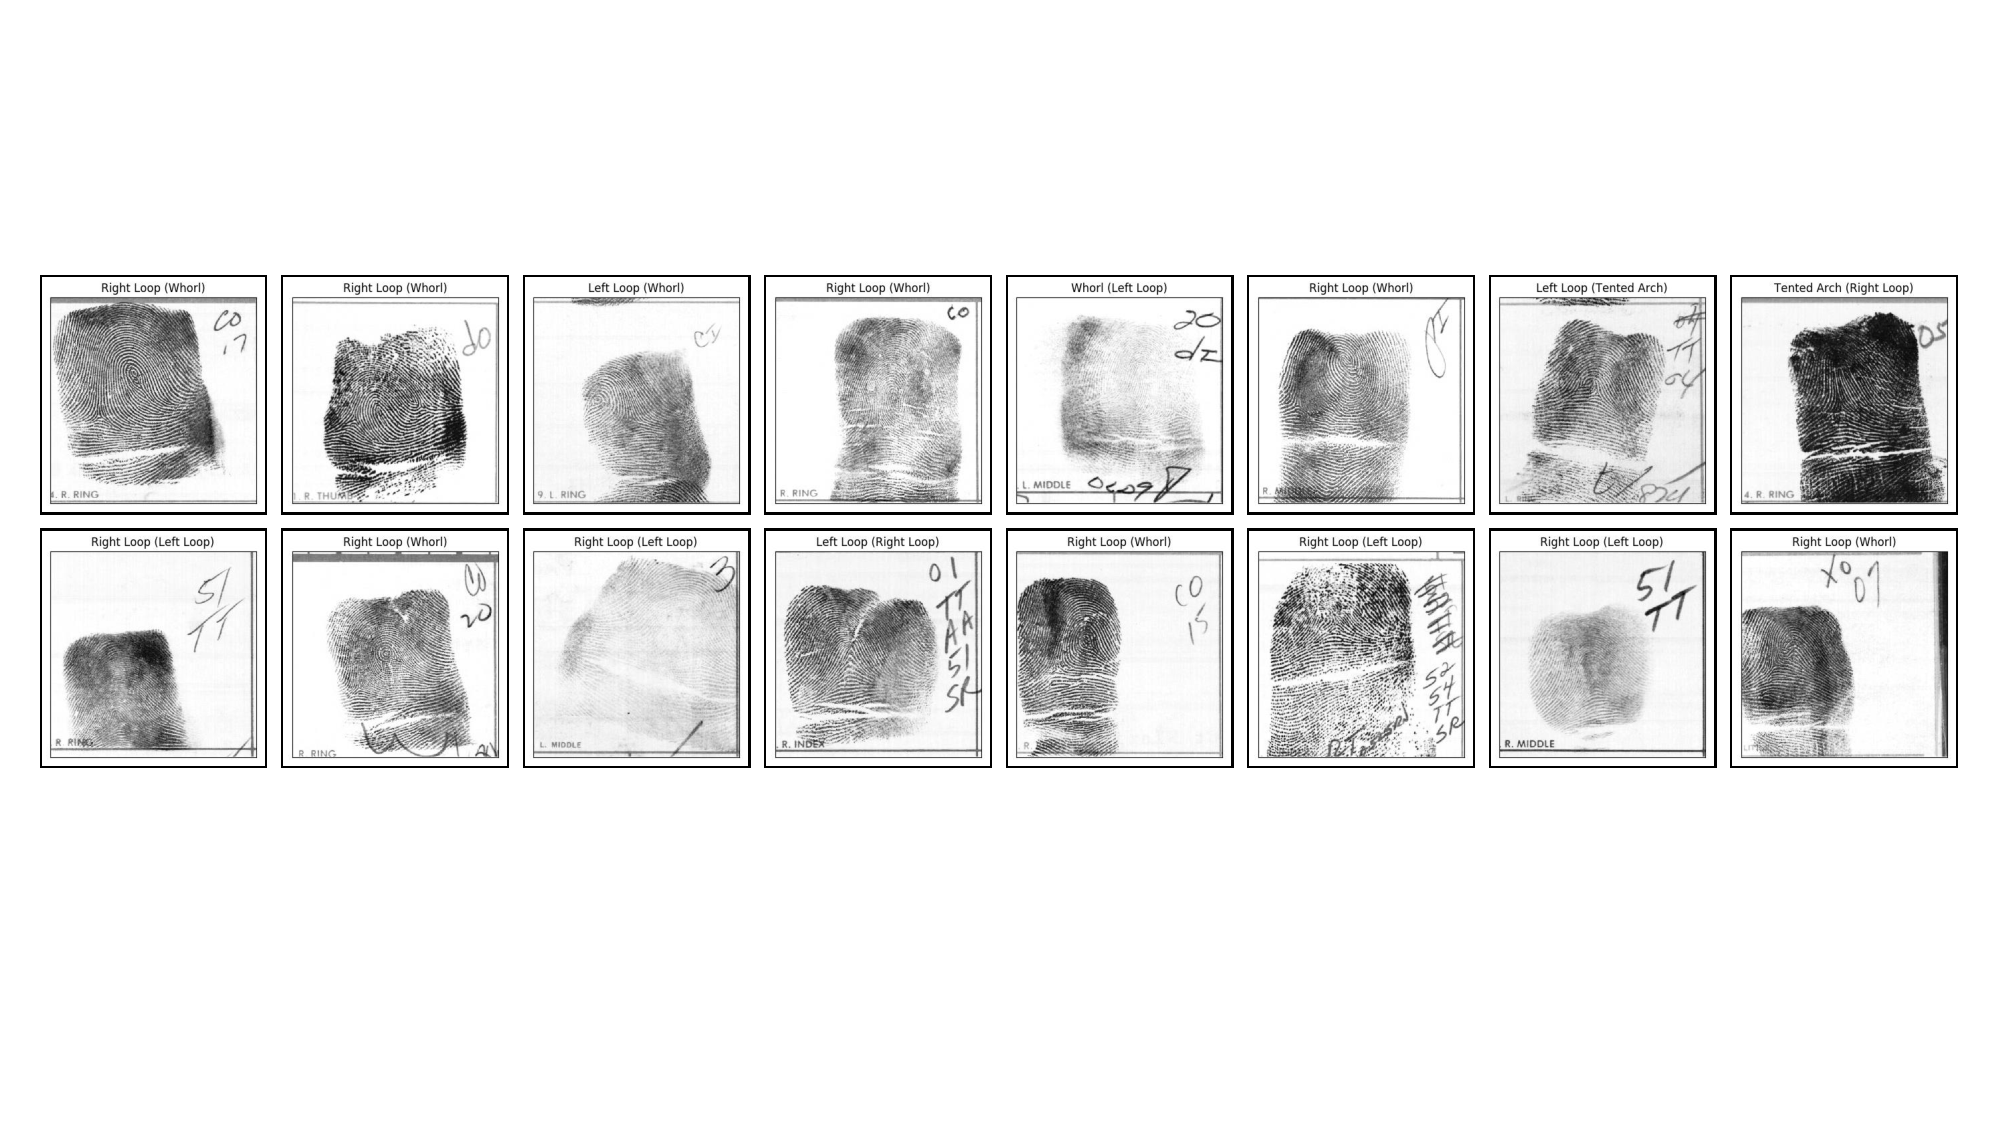
\includegraphics[scale=0.53,clip=true,trim = 5mm 60mm 5mm 45mm]{fig/figs/fail.pdf}
	\end{center}
	\caption{Mis-classification examples on NIST SD14. The title of each example is \textit{Prediction}(\textit{Ground Truth})} 
	\label{fig.fails}
\end{figure*}





\section{Conclusion and Future Work}
\label{sec_con}
%!TEX root = main.tex

In this paper, we propose a deep learning approach for automatic fingerprint type classification. We design a deep ConvNet based on residual network. To preserve as much fingerprint details as possible, the input image is designed to be  $512\times512$ and we can use two early convolutional layers to reduce the computational cost. The deep ConvNet serves as a feature extractor and on top of that a SVM is trained as the final classifier. Experiment results show that the proposed automatic that does not rely on any hand-crafted features can achieve high accuracy comparable to the state-of-the-art approach even if only label is used. Our proposed can accurately predict the fingerprint class using raw images, avoiding the need of using orientation filed estimation. Future works include using more advanced deep networks and ensemble techniques to fuse multiple classifiers.



{\small
\bibliographystyle{ieee}
\bibliography{ijcb2017_main}
}

\end{document}
